\documentclass[12pt,a4paper]{article}
%-----------------------PACKAGES-----------------------%
\usepackage[top=1in,bottom=1in,left=0.5in,right=0.5in]{geometry}
\usepackage{graphicx}
\usepackage{array}
\usepackage{xcolor}
\usepackage{adjustbox}
\usepackage{titlesec}
\usepackage{svg}
\usepackage{lettrine}

%-----------------------TABLES ALIGNEMNET-----------------------%

%-----------------------TITLE DOCUMENT-----------------------%
\begin{document}
	\begin{Titlepage}
\begin{center}
    \vspace*{2cm}
    
    \textbf{\Huge The Web Artisan}\\
    \vspace*{2cm}
    
       \textbf{ \large Group-Member}
      \vspace{0.2cm}
      \begin{center}
          \large Maria 19F-0908\\Iradat 19F-0977\\Wahaj 19F-1014
      \end{center} 
    
    \vspace{1.5cm}
    \begin{center}
    \large April,2023 
    \end{center}
    
    \vfill
    \vspace{0.8cm}
    \begin{figure}[hb]
        \centering
        
\includegraphics[scale=0.20]{Files/Fast-Nuces.png}
    \end{figure}
    Department of Computer Science\\ National University of Computer and Emerging Science\\ Chiniot Faisalabad Campus, Pakistan 2023
    \end{center}
\end{Titlepage}









 
 \clearpage
%-----------------------TABLE OF CONTENT-----------------------% 
\tableofcontents
\clearpage
%-----------------------TABLE OF CONTENT-----------------------% 
\section{Need of the Project}
\lettrine[findent=2pt]{\fbox{\textbf{T}}}{}oday everyone is entering digital era. The brands are moving to online platforms to target a great number of audiences that is sitting online. So outsource is an IT company which provides computerized advertising Services in Pakistan and yielding procedures to convey the clients with high caliber and viable I.T benefits in Pakistan.
\section{Situation Analysis}
\subsection{SWOT Analysis}
It stands for Strengths, Weaknesses, Opportunities, and Threats.
\subsubsection{Strengths}
\begin{itemize}
    \item Strong technical expertise and experience in web design and development.
    \item Good reputation and positive customer reviews, which can lead to referral business.
    \item A diverse portfolio of clients across different industries.
    \item Flexibility in terms of offering both custom and template-based solutions.     
\end{itemize}
\subsubsection{Weaknesses}
\begin{itemize}
    \item Heavy reliance on a few key clients for revenue.
    \item Limited marketing and brand awareness, which can limit potential customer reach.
    \item High competition in the web design and development industry, which can make it challenging to stand out.  
    \item Potential difficulties in maintaining quality as the business scales up.
\end{itemize}
\subsubsection{Opportunities}
\begin{itemize}
    \item Expansion into new geographic regions or markets.
    \item Developing new service offerings, such as mobile app development or search engine optimization (SEO).
    \item Leveraging social media and content marketing to increase brand awareness and attract new clients.
    \item Offering specialized services for niche industries or target markets.
\end{itemize}
\subsubsection{Threats}
\begin{itemize}
    \item Economic downturns or recessions, which can lead to reduced demand for web design and development services.
    \item Rapid changes in technology, which can require significant investments in training or new equipment.
    \item Intense competition from other web design and development companies, including larger and more established firms.
    \item Changing consumer preferences or shifts in the way businesses approach marketing and customer engagement.
\end{itemize}
\subsection{PEST}
It stands for Political, Economic, Social, and Technological factors.
\subsubsection{Political Factors}
\begin{itemize}
    \item There are no specific political factors that impact the pest situation of web Artisan.
    \item However, local and regional regulations may impact the use of pesticides to control web artisan, and their impact on the environment.    
\end{itemize}
\subsubsection{Economics Factor}
\begin{itemize}
    \item Web Artisan can cause economic damage to crops and structures, leading to losses for farmers, property owners, and businesses.
    \item Pest control services for web Artisan can also be costly and may impact the bottom line for businesses and individuals.    
\end{itemize}
\subsubsection{Social Factor}
\begin{itemize}
    \item People generally dislike the presence of web Artisan, as they can be unsightly and cause fear or discomfort.
    \item Web Artisan may also impact the health and well-being of humans and animals, such as causing allergic reactions or attracting other pests like spiders.
\end{itemize}
\subsubsection{Technological Factor}
\begin{itemize}
    \item New pest control technologies, such as biological controls or precision pesticides, may offer more targeted and sustainable methods of controlling web Artisan.
    \item However, web Artisan themselves are not necessarily influenced by technological factor.Overall, the pest situation of web Artisan is primarily driven by economic and social factors, with potential regulatory impacts. The use of new technologies may offer more effective and sustainable control methods in the future.
\end{itemize}
\section{Market Analysis}
\subsection{Segmentation}
\subsubsection{Geographic Segmentation}
Web Artisan can be found in a variety of geographic locations, but their prevalence and impact may vary depending on the climate, vegetation, and structures in the area. For example, web Artisan may be more common in humid regions with abundant vegetation, or in areas with older buildings that provide more favorable nesting sites. Pest control companies and property owners may need to consider these geographic factors when developing strategies for managing web Artisan.
\subsubsection{Demographic Segmentation}
There is no specific demographic group that is more or less susceptible to the presence of web Artisan. However, certain demographic factors may impact the level of concern or willingness to take action against web Artisan. For example, property owners who are more house-proud or concerned about the appearance of their homes may be more likely to seek out pest control services for web Artisan. Similarly, people with allergies or other health concerns may be more motivated to eliminate web Artisan from their living spaces.
\subsubsection{Psychographic Segmentation}
 Psychographic segmentation refers to the personality traits, attitudes, and values of consumers. When it comes to web Artisan, different individuals may have different levels of tolerance for these pests. For some people, web Artisan may be seen as an interesting natural phenomenon, while for others they may be a source of fear or discomfort. Pest control companies may need to take these psychographic factors into account when developing marketing messages or outreach strategies.
\subsubsection{Behavioral Segmentation}
Behavioral segmentation looks at the actions and behaviors of consumers. In the case of web Artisan, property owners or businesses may exhibit different behaviors depending on their level of concern or awareness of the issue. For example, some property owners may proactively seek out pest control services as soon as they notice web Artisan, while others may wait until the problem becomes more severe. Pest control companies may need to tailor their services and messaging based on the behavior of their target customers.
\subsection{Targeting}
The target market for pest control services related to web Artisan would primarily consist of property owners, including homeowners, business owners, and managers of public spaces like parks and gardens. These individuals are likely to have a vested interest in maintaining a clean and pest-free environment, and may be willing to pay for services that help to eliminate web Artisan from their properties.
\subsubsection{Targeting Strategies}
\begin{itemize}
    \item Geographic Targeting: Companies may target specific geographic regions where web Artisan are particularly prevalent or problematic. For example, companies operating in areas with high humidity or older buildings may focus their marketing efforts in those regions.
    \item Psychographic Targeting: Companies may target individuals with specific attitudes or values related to cleanliness, aesthetics, or health. For example, companies may target homeowners who place a high value on the appearance of their homes, or parents who are concerned about the potential health impacts of web Artisan on their children.
    \item Behavioral Targeting: Companies may target individuals who have exhibited specific behaviors related to web Artisan, such as searching for information about web Artisan online, or contacting pest control companies for help with a web weaver infestation.
    \item Advertising and Promotions: Companies may use a variety of advertising and promotional strategies to reach their target market, including social media ads, local print ads, direct mail, and referral programs.
\end{itemize}
\subsection{Differentiation}
\subsubsection{Differentiation Strategies}
\begin{itemize}
    \item Differentiation strategies are focused on highlighting the unique value or benefits of a product or service compared to competitors. In the case of web Artisan, differentiation strategies for pest control services could include:
    \item Environmentally-Friendly Pest Control: Pest control companies could differentiate themselves by offering environmentally-friendly methods of controlling web Artisan, such as natural predators or biological controls. This could appeal to consumers who are concerned about the use of pesticides or other harmful chemicals.
    \item Customized Pest Control Plans: Companies could differentiate themselves by offering customized pest control plans based on the unique needs and preferences of each customer. For example, some customers may prefer a more aggressive approach to eliminating web Artisan, while others may prefer a more natural approach.
    \item Professional Expertise: Companies could differentiate themselves by emphasizing their professional expertise in the field of pest control. This could include highlighting the training and experience of their technicians, as well as their use of the latest pest control technologies and techniques. Guarantee of Results: Companies could differentiate themselves by offering a guarantee of results for their pest control services. This could give customers greater confidence in the effectiveness of the company's services, and could also help to build trust and loyalty over time.
\end{itemize}
\subsubsection{Target Market}
The target market for differentiated pest control services related to web Artisan would primarily consist of property owners, including homeowners, business owners, and managers of public spaces like parks and gardens. These individuals are likely to have a vested interest in maintaining a clean and pest-free environment and may be willing to pay for services that offer unique value or benefits compared to competitors.
\subsection{Positioning}
\begin{itemize}
    \item Identify the target market: The first step in any market analysis is to identify the target market. For web Artisan, this may include small businesses, startups, or individuals who need a website or web application developed. It's important to understand the demographics, psychographics, and behaviors of the target audience to better tailor the marketing message.
    \item Identify the competition: In order to position web Artisan effectively, it's important to understand who the competition is and what they offer. This can be done through a competitive analysis, where web Artisan can evaluate the strengths and weaknesses of their competitors, and determine how they can differentiate themselves.
    \item Determine the unique selling proposition: Based on the competitive analysis, web Artisan can determine their unique selling proposition (USP) – the factor that sets them apart from their competitors. This could be anything from the quality of their work, their pricing, their customer service, or their expertise in a particular niche.
     \item Develop the marketing message: Once the USP has been identified, web Artisan can develop a marketing message that resonates with the target audience. This could include highlighting the USP in all marketing materials, such as the website, social media, and advertising.
      \item Choose the marketing channels: Finally, web Artisan need to choose the right marketing channels to reach their target audience. This could include online channels such as search engine optimization (SEO), social media, email marketing, or paid advertising, as well as offline channels such as networking events or print advertising.
\end{itemize}
By applying a positioning analysis, web Artisan can differentiate themselves in the crowded web development market and better reach their target audience with a compelling marketing message.
\section{Four P's}
As a web artisan, We can fulfill the Four P's for web application by considering the following
\subsection{Product}
Determine what features and functionalities web application will offer and how you can differentiate it from competitors. Develop a user interface and user experience that aligns with the target audience and their needs.
\begin{itemize}
    \item Identify the problem web Artisan will solve: Determine the specific pain points your target audience faces and develop features and functionalities that address those problems.
    \item Research competitors: Analyze what your competitors are offering and identify gaps in the market that you can fill with web Artisan. Differentiate your application by offering unique features or by providing a better user experience.
    \item Focus on user experience: Ensure that the user interface is intuitive and easy to use. Focus on user-centered design principles and conduct user testing to improve the user experience.
    \item Consider scalability: Determine that web Artisan needs to scale as the user base grows. Ensure that your application is designed to handle increased traffic and user demand.
    \item Leverage technology: Consider using the latest technologies to provide a unique experience for your users. For example, you could use artificial intelligence or machine learning to offer personalized recommendations or to automate certain tasks.
    \item Continuously update and improve: Keep track of user feedback and make updates and improvements to your web application regularly to ensure that it continues to meet the needs of your target audience.
\end{itemize}
By considering these factors, you can develop a web Artisan that offers unique features and functionalities and provides a superior user experience, which can help you differentiate your application from competitors.
\subsection{Price}
Determine the pricing strategy for web Artisan, whether it's a subscription fee, a one-time fee, or a free application with in-app purchases or advertising. Ensure that the pricing strategy aligns with the value proposition of the application and the target audience.
\subsection{Place}
Determine the distribution channels to reach your target audience, including the web, app stores, social media platforms, and other relevant platforms. Ensure that the distribution channels align with the target audience and the marketing goals of the application.
\begin{itemize}
    \item Identify your target audience: Determine who your target audience is and where they spend their time online. This will help you understand which distribution channels are most effective for reaching them.
    \item Research distribution channels: Identify the distribution channels that are most relevant to your target audience, such as the web, app stores, social media platforms, and other relevant platforms. Research which channels are most commonly used by your target audience and analyze which ones are most effective for your application.
    \item Analyze the competition: Research how competitors are distributing their web applications and identify which channels they are using to reach their target audience. This can give you insight into which channels are most effective for your market.
    \item Consider marketing goals: Determine what marketing goals are and how they align with your distribution channels. For example, if your goal is to build brand awareness, social media platforms may be a good distribution channel. If your goal is to generate revenue, app stores or subscription models may be more effective.
    \item Test and measure: Once you have identified your distribution channels, test and measure the effectiveness of each channel. Use analytics to track user behavior and conversion rates and adjust your distribution strategy accordingly.
\end{itemize}
\subsection{Promotion}
Determine the marketing activities to raise awareness and attract users to web Artisan, including online advertising, content marketing, search engine optimization, social media marketing, and influencer marketing. Ensure that the promotion strategy aligns with the target audience and the marketing goals of the application.
\begin{itemize}
    \item Define your target audience: Understand who your target audience is and what channels they use to discover new products or services. This will help you determine which marketing activities are most effective in reaching them.
    \item Set marketing goals: Identify marketing goals, such as increasing brand awareness, driving traffic, generating leads, or increasing revenue. These goals will help you determine which marketing activities align with your objectives.
    \item Choose marketing channels: Consider different marketing channels that align with your target audience and marketing goals, such as online advertising, content marketing, search engine optimization, social media marketing, or influencer marketing. Choose the channels that are most effective in reaching your target audience and promoting your web application.
    \item Develop marketing content: Create high-quality content that resonates with your target audiences, such as blog posts, social media posts, videos, or infographics. Ensure that the content is relevant, informative, and aligned with your marketing goals.
    \item Plan and execute campaigns: Develop a campaign strategy that includes specific tactics, timelines, and budgets. Execute the campaigns across different channels and measure the results using analytics tools.
    \item Optimize and refine: Continuously track and analyze the performance of our  marketing campaigns, and refine them based on the results. Identify what works and what doesn't and optimize your strategy accordingly.
\end{itemize}
\section{Business Analysis}
\begin{itemize}
    \item Identify the business problem: Determine the problem that the web Artisan is trying to solve. 
    \item Gather and document business requirements: Collect the business requirements for the web Artisan by engaging with stakeholders such as users, customers, and business owners. Document these requirements in a clear and concise manner.
    \item Conduct a feasibility study: Determine the feasibility of developing the web Artisan by analyzing factors such as technical feasibility, economic viability, and operational feasibility.
    \item Create a functional specification: Develop a functional specification that describes the features, functionality, and user experience of the web Artisan. 
    \item Develop a project plan: Create a project plan that outlines the timeline, budget, and resources required for developing the web Artisan. 
    \item Conduct a risk analysis: Identify the risks associated with developing and deploying the web Artisan, and develop strategies to mitigate these risks.
    \item Conduct user acceptance testing: Test the web Artisan with users to ensure that it meets their needs and is easy to use. Use feedback from user testing to make improvements to the web Artisan.
\end{itemize}
\subsection{Promotional budget}
We will provide you 2 Week free support after launching the project
\begin{itemize}
    \item We are responsible for our design, development and coding bug
    \item Any bug or problem will be solve free of cost during the support time
    \item Monthly Management Fee Will be Rs 25000 Pkr
    \item Enhancing your product and make it better day by day
    \item Creative Post Design
    \item Posts per Week
    \item Advertising
    \item 1 Video Per Month
    \item Content Management
    \item Social Media Management
    \item Website Management of high traffic 
    \item Website Up-time 24/7
    \item Technology Up-gradation to new version and make it compatible with running product with 0 downtime
    \item Any Development and the new feature will be charged separately 
\end{itemize}
\subsection{Projected income statement for 3 years}
\begin{table}[h!]
\caption{Projected income statement for 3 years}
    \centering
    \begin{tabular}{|p{10cm}|p{3cm}|p{3cm}|}
    \hline
       \textbf{Description}  &\textbf{Net Amount} &\textbf{Time Frame}  \\%end of row
       \hline
        Advance Payment  &30\% &\textbf{-} \\%end of row
       \hline
        Prototype Approval  & 30\%&7 Working Days \\%end of row
       \hline
        Final Delivery &40\%&-\\%end of row
       \hline
        \textbf{Total Cost}  &\textbf{-} & \\%end of row
       \hline
    • This quotation is valid for a period of days from the date of issue.
    \newline • Terms of payment are 30\% upon approval of this proposal, 30\% of design structure approval, and the remaining 40\% upon completion of the project.& &\\ 
      \hline       
    \end{tabular}
\end{table}
\clearpage
\section{Project Poster and Flex}
    \begin{figure}[h!]
        \centering
        
\includegraphics[scale=0.20]{Files/POSTER.png}
    \end{figure}
    \begin{figure}[h!]
        \centering
        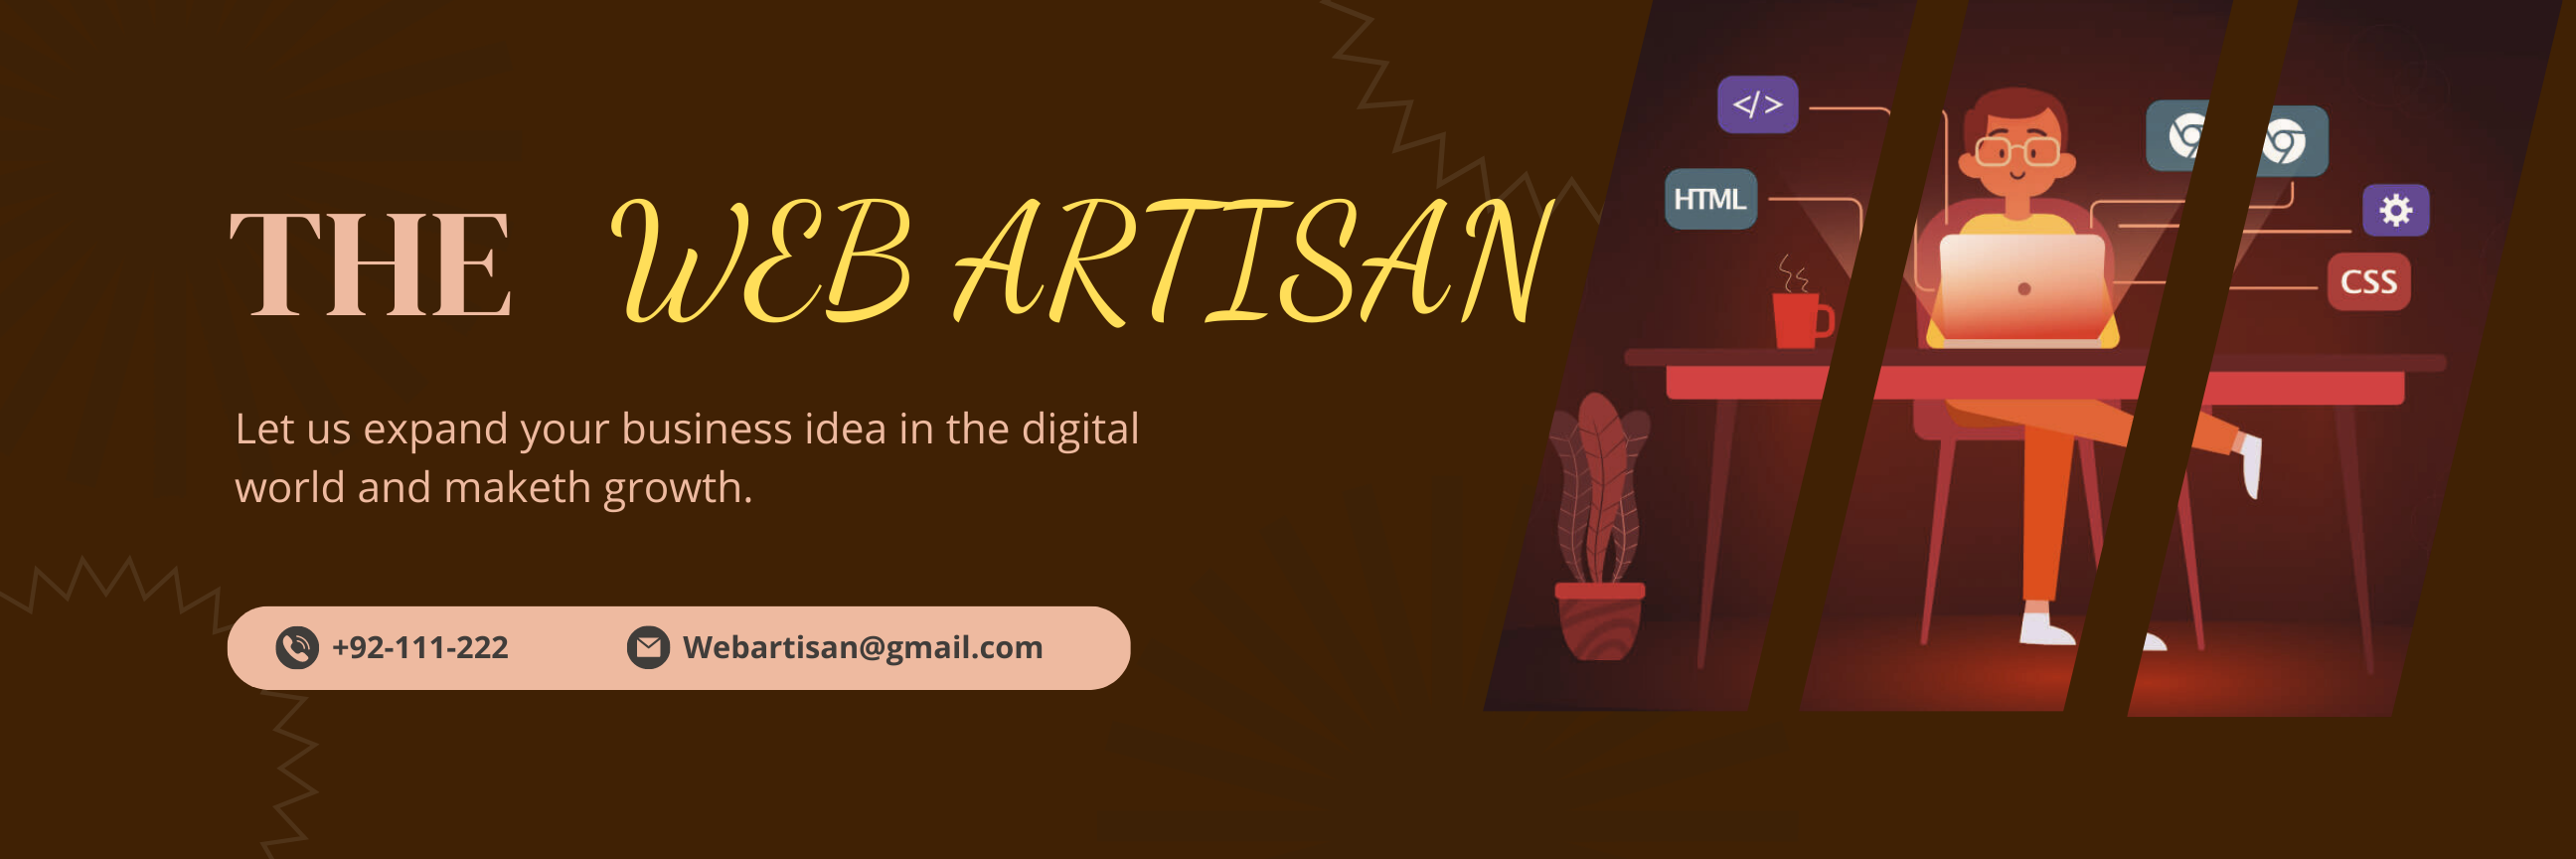
\includegraphics[scale=0.20]{Files/FLEX.png}
    \end{figure}



\end{document}